\documentclass[a4paper,11pt]{article}
\pdfoutput=1 % if your are submitting a pdflatex (i.e. if you have
             % images in pdf, png or jpg format)
\usepackage{jheppub} % for details on the use of the package, please
                     % see the JHEP-author-manual
\usepackage[T1]{fontenc} % if needed

\usepackage{wrapfig,lipsum,booktabs}
\usepackage{pdflscape}
\usepackage{latexsym}
\usepackage{epsfig}
\usepackage[mathscr]{eucal}
\usepackage{amsfonts}
\usepackage{amscd}
\usepackage{amsmath}
\usepackage{array}
\usepackage{amssymb}
\usepackage{colordvi}
\usepackage{enumerate}
\usepackage{graphicx}
\usepackage{booktabs}
\usepackage[footnotesize]{caption}
\usepackage{fancyhdr} 
\usepackage{pdfpages}
\usepackage{slashed}
\usepackage{tabularx}
\usepackage{longtable}
\usepackage{array}
\usepackage{relsize}
\usepackage{color}
\usepackage{rotating}
\usepackage{slashed}
\usepackage{subfigure}
\usepackage{xspace}
\usepackage{booktabs}
\usepackage{epsfig,amsmath,graphicx,amssymb,listings,slashed}
\usepackage[colorlinks,citecolor=blue,urlcolor=blue,linkcolor=blue]{hyperref}

\title{{\boldmath Validation Note for the MadAnalysis 5 implementation of the Analysis ATLAS-CONF-2019-040}}

\newcommand{\MG}{{\sc MadGraph5\textunderscore}a{\sc MC@NLO}}
\newcommand{\PY}{{\sc Pythia\,8.230}\xspace}
\newcommand{\DEL}{{\sc Delphes\,3\xspace}}

\author[a,]{Federico Ambrogi,\note{Corresponding author.}}


% The "\note" macro will give a warning: "Ignoring empty anchor..."
% you can safely ignore it.

\affiliation[a]{Department of Meteorology and Geophysics, University of Vienna, Vienna, Austria}


% e-mail addresses: one for each author, in the same order as the authors
\emailAdd{federico.ambrogi@univie.ac.at}

%\abstract{}

\begin{document} 
	\maketitle
	\flushbottom
	\section{Introduction}
	We present here the validation of the MadAnalysis  5\cite{Dumont:2014tja, Conte:2014zja, Conte:2018vmg} v1.7 implementation of the analysis ATLAS-CONF-2019-040\cite{ATLAS2019vcq} by the ATLAS Collaboration, which searches for Supersymmetry (SUSY) with proton-proton collisions at the LHC. The analysis focusses on final states with large hadronic activity. The base requirement for at least two jets with high transverse momentum and no isolated energetic leptons makes the analysis sensitive to many possible SUSY scenarios which, in particular models with production of gluinos and squarks. 
	\\	
	Similar analyses performed at different centre-of-mass energy or total luminosity of the dataset (ATLAS-SUSY-2013-02\cite{Aad:2014wea} and ATLAS-SUSY-2016-07\cite{Aaboud:2017vwy}) were also implemented and validated in the MadAnalysis 5 framework (\cite{ATLAS-SUSY-2013-02MA5} with \cite{ATLAS-SUSY-2013-02VALIDATION}, \cite{ATLAS-SUSY-2016-07MA5} with \cite{ATLAS-SUSY-2016-07VALIDATION}). The preliminary results published in ATLAS-CONF-2019-040 are based on collisions performed at 13 TeV centre-of-mass energy and uses a total integrated luminosity of 139 $fb^{-1}$. 
	%The analysis is made available in the MadAnalysis 5 Public Analysis Database \cite{MA5PAD}. 
	The search presented in ATLAS-CONF-2019-040 utilizes three different strategies. The first defines search regions which are mutually orthogonal, hence can be statistically combined to derive cross section upper limits. The second strategy uses boosted decision trees for event selection, while the third approach, based on a classic cut-and-count selection of events,
	is the one we implemented that we will to discuss. \\
	
	The cut-and-count strategy is based on the selection of events which exhibits large momentum imbalance of the visible particle, i.e. large missing transverse energy $E_T^{miss}$. Isolated leptons, with pseudorapidity $|\eta|<$2.7 (2.47) are vetoed if $p_T>$6(7) GeV respectively for muons or electrons.
	Signal jets must have $p_T>$50 GeV and a pseudorapidity $|\eta|<$2.8 . 
	A large amount of hadronic activity, in the form of large jets multiplicity $n_j$ and large values of the missing hadronic transverse $H_T$ (scalar sum of all signal jets momenta) is required in the events, as well as large values of the "effective mass" variable calculated as $m_{eff}= H_T + E_T^{miss}$.
	\\
	
	Ten different search regions, targetting specific simplified model signatures, are then designed by applying cuts on the jet multiplicity, jet angular separation, jet momenta, pseudorapidity, hadronic transverse energy and effective mass. This way, the same events might belong to several overlapping signal regions. A precise definition of the cuts can be read in the validation tables in Section \ref{sec::validation}. 
	
	\section{Monte Carlo Samples Generation}
	Following the procedure adopted by the ATLAS collaboration, we produced the SUSY signals of interest using \MG~\cite{Alwall:2014hca} to generate events at parton level, with the inclusion of up to 2 additional extra partons. The events where then showered and hadronized using \PY~\cite{Sjostrand:2014zea}. The matching and merging between the matrix element and the parton shower formalism was obtained running the script main89.cc included in \PY~, using the CWKKL algorithm. The CWKKL merging scale was set to 1/4 of the mass of the SUSY particles produced in the collision up to the value of 500 GeV.  
	The simulation of ATLAS detector was performed by \DEL~\cite{deFavereau:2013fsa}, using an adapted simulation card that was already used for the previous validation of the analysis ATLAS-SUSY-2016-07. Jets were reconstructed using the FastJet algorithm \cite{Cacciari:2011ma}, using the anti-\textit{k}$_T$\cite{Cacciari:2008gp} jet clustering algorithm with a jet radius parameter equal to 0.4.     
	
	\section{Validation}\label{sec::validation}
	In this section we compare the results obtained with our implementation of the analysis and a series of cut-flow tables provided by the ATLAS collaboration, both on the wiki page of the analysis and the preliminary document. Official results are interpreted with four different simplified models:
	\begin{itemize}
	\item gluino with direct decay: $p p \rightarrow \tilde q \tilde q , \tilde q \rightarrow q \tilde \chi _1 ^0$ \
	\item gluino with one-step cascade decay:  $p p \rightarrow \tilde g \tilde g , \tilde g \rightarrow qq'  \tilde \chi _1 ^{\pm} , \tilde \chi _1 ^{\pm} \rightarrow W^{\pm} \tilde \chi _1 ^0$ \
	\item squark with direct decay: $p p \rightarrow \tilde q \tilde q , \tilde q \rightarrow q \tilde \chi _1 ^0$ \
	\item squark with  one-step cascade decay: $p p \rightarrow \tilde q \tilde q , \tilde q \rightarrow q'  \tilde \chi _1 ^{\pm} , \tilde \chi _1 ^{\pm} \rightarrow W^{\pm} \tilde \chi _1 ^0$ \
	\end{itemize}
	
	The simplified models for gluinos consider the direct 3-body decays of gluinos to a pair of jets and the neutralinos, and the decays of gluinos to the neutralinos via a 1-step cascade decay, with an intermediate chargino. Similarly, the squark simplified models consider the direct decays of the squark to the neutralino and a standard model quark, or the intermediate decay to a different flavour quark and a chargino, decaying to a W boson and the neutralino. The diagrams are depicted in Fig. \ref{sms}. All the squarks belonging to the first two families, both with left and right helicities, are considered for the model with direct decays; only left-handed squarks are considered in the case of the one-step cascade decay model.
	In the following sections, the comparison with the ATLAS and MA5 cutflow tables are shown; we rescaled the number of events obtained with MA5 in the top row to match the first number in the ATLAS tables.
	
	\begin{figure}
		\begin{center}
			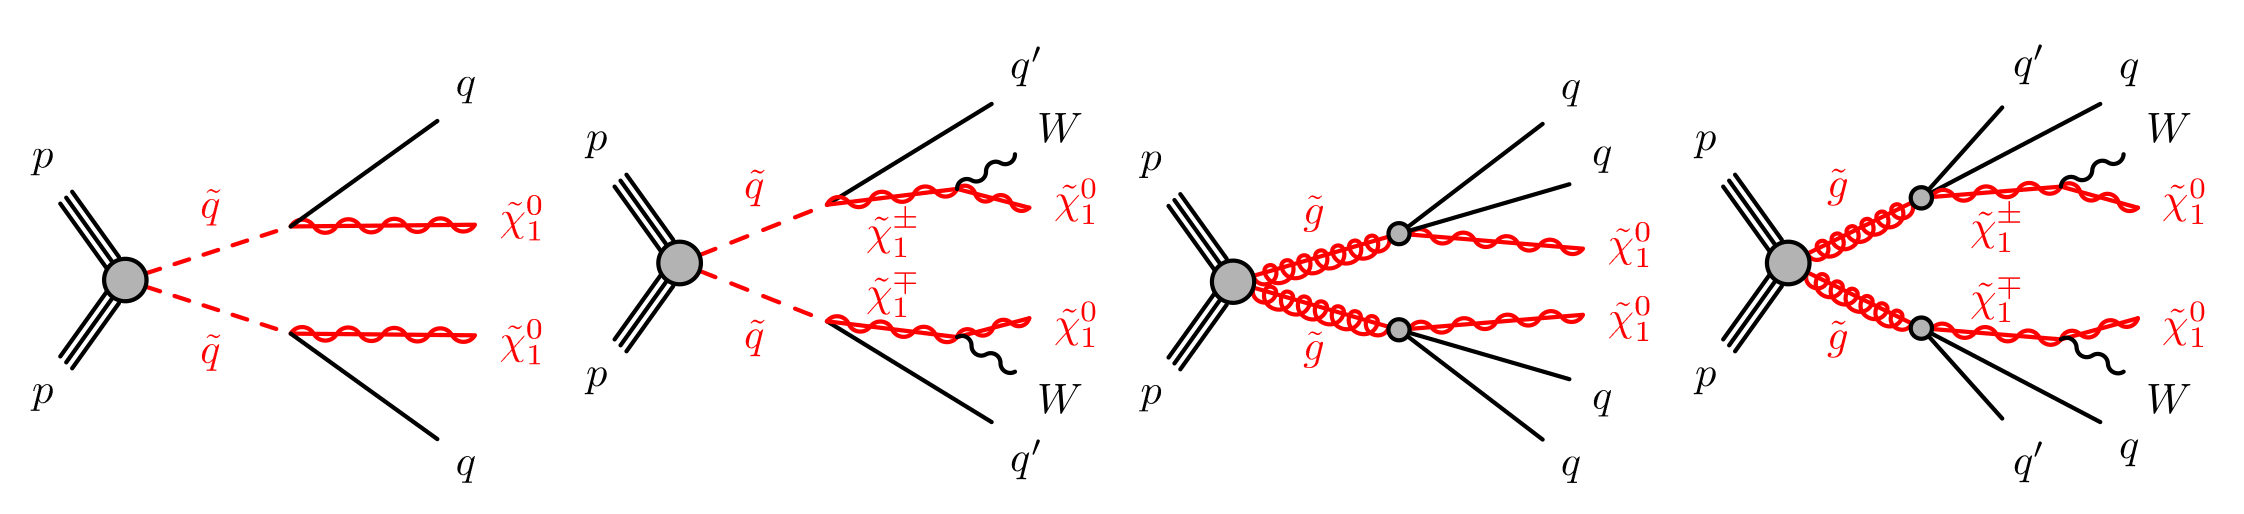
\includegraphics[width=1\textwidth]{sms.png}	
		\end{center}
		\caption{Diagrams for the simplified models used for the validation of the implementation: from left, squark model with direct decay; squark model with 1-step decay; gluino model with direct decay; gluino model with 1-step decay. Taken from \cite{ATLAS2019vcq}.}
		\label{sms}
	\end{figure}


	\clearpage
			\begin{landscape}
	\subsection{Squark model: $p p \rightarrow \tilde q \tilde q , \tilde q \rightarrow q \tilde \chi _1 ^0$}


	\begin{table}[h]
		\centering
		\renewcommand\arraystretch{1.2} 
		\scriptsize
		\begin{tabular}{ | l | c c c c  || c c c c || c c c c | } \toprule
			%\toprule \toprule
			%\multicolumn{3}{c}{($M_1,M_2,M_3) = (1200,600,500)$} & %\multicolumn{3}{c}{ \textbf{T3GQ}} & \multicolumn{3}{c}{ %\textbf{T3QG}} \\  \toprule 
 $(m_{\tilde q},m_{\tilde \chi _1 ^0})$ &	\multicolumn{4}{c}{\textbf{(1200,600)}} & \multicolumn{4}{c}{\textbf{(1400,600)}} &
 \multicolumn{4}{c|}{\textbf{(1600,400)}} \\ \hline 
 		
			\textbf{Cut} & \textbf{ATLAS} & $\%$ & \textbf{MA5} & $\%$ & \textbf{ATLAS} & $\%$ & \textbf{MA5} & $\%$ & \textbf{ATLAS} & $\%$ & \textbf{MA5} & $\%$ \\ \hline \hline


\multicolumn{13}{|l|}{\textbf{SR2j-1600}} \\ \hline
Preselection&1763.0&&1763.0&&541.0&&541.0&&174.0&&174.0&
\\
$n_j>$2&1763.0&0.0&1763.0&0.0&541.0&0.0&541.0&0.0&174.0&0.0&174.0&0.0
\\
$\Delta \phi(j_{1,2,(3)},\mathbf{p}_T^{miss})>$0.8&1433.0&-18.7&1413.5&-19.8&431.0&-20.3&435.0&-19.6&136.0&-21.8&136.5&-21.5
\\
$\Delta \phi(j_{i>3},\mathbf{p}_T^{miss})>$0.4&1377.0&-3.9&1354.4&-4.2&411.0&-4.6&411.3&-5.5&129.0&-5.1&129.2&-5.4
\\
$p_T(j_2)>$250 GeV &853.0&-38.1&854.6&-36.9&311.0&-24.3&316.0&-23.2&111.0&-14.0&111.0&-14.1
\\
$|\eta(j_{1,2})|<2$&836.0&-2.0&837.3&-2.0&306.0&-1.6&310.6&-1.7&109.0&-1.8&108.2&-2.5
\\
$E_T^{miss}/\sqrt{H_T}>16 $ GeV$^{1/2}$&568.0&-32.1&567.8&-32.2&228.0&-25.5&229.2&-26.2&86.4&-20.7&85.8&-20.7
\\
$m_{eff}>$1600 GeV&366.0&-35.6&379.5&-33.2&202.0&-11.4&201.8&-12.0&83.5&-3.4&83.0&-3.2
\\ \hline

\multicolumn{13}{|l|}{\textbf{SR2j-2200}} \\ \hline
Preselection&1763.0&&1763.0&&541.0&&541.0&&174.0&&174.0&
\\
$n_j>$ 2&1763.0&0.0&1763.0&0.0&541.0&0.0&541.0&0.0&174.0&0.0&174.0&0.0
\\
$\Delta \phi(j_{1,2,(3)},\mathbf{p}_T^{miss})>$0.4&1603.0&-9.1&1593.1&-9.6&483.0&-10.7&490.8&-9.3&156.0&-10.3&154.9&-11.0
\\
$\Delta \phi(j_{i>3},\mathbf{p}_T^{miss})>$0.2&1567.0&-2.2&1561.4&-2.0&470.0&-2.7&476.7&-2.9&151.0&-3.2&150.2&-3.0
\\
$p_T(j_1)>$600 GeV&509.0&-67.5&521.4&-66.6&269.0&-42.8&270.7&-43.2&120.0&-20.5&119.6&-20.4
\\
$E_T^{miss}/\sqrt{H_T}>$16 GeV$^{1/2}$&337.0&-33.8&350.7&-32.7&201.0&-25.3&200.1&-26.1&94.6&-21.2&94.1&-21.3
\\
$m_{eff}>$2200 GeV&101.0&-70.0&99.6&-71.6&108.0&-46.3&108.0&-46.0&76.1&-19.6&77.4&-17.8
\\ \hline
\multicolumn{13}{|l|}{\textbf{SR2j-2800}} \\ \hline
Preselection&1763.0&&1763.0&&541.0&&541.0&&174.0&&174.0&
\\
$n_j>$ 2&1763.0&0.0&1763.0&0.0&541.0&0.0&541.0&0.0&174.0&0.0&174.0&0.0
\\
$\Delta \phi(j_{1,2,(3)},\mathbf{p}_T^{miss})>$0.8&1433.0&-18.7&1413.5&-19.8&431.0&-20.3&435.0&-19.6&136.0&-21.8&136.5&-21.5
\\
$\Delta \phi(j_{i>3},\mathbf{p}_T^{miss})>$0.4&1377.0&-3.9&1354.4&-4.2&411.0&-4.6&411.3&-5.5&129.0&-5.1&129.2&-5.4
\\
$p_T(j_2)>$250 GeV &853.0&-38.1&854.6&-36.9&311.0&-24.3&316.0&-23.2&111.0&-14.0&111.0&-14.1
\\
$|\eta(j_{1,2})|$<1.2&655.0&-23.2&657.1&-23.1&235.0&-24.4&241.6&-23.5&82.3&-25.9&84.6 &-23.8
\\
$E_T^{miss}/\sqrt{H_T}>16 $ GeV$^{1/2}$&439.0&-33.0&442.5&-32.6&173.0&-26.4&177.3&-26.6&64.6&-21.5&67.0&-20.8
\\
$m_{eff}>$2800 GeV&15.6&-96.4&15.5&-96.5&18.8&-89.1&17.5&-90.1&29.1&-55.0&29.8&-55.5
\\





			\bottomrule \bottomrule
		\end{tabular}

\end{table}	
		
		\end{landscape}
	
	\clearpage
	\subsection{Squark model: $p p \rightarrow \tilde q \tilde q , \tilde q \rightarrow q'  \tilde \chi _1 ^{\pm} , \tilde \chi _1 ^{\pm} \rightarrow W^{\pm} \tilde \chi _1 ^0$}
	
		\begin{table}[h]
		\centering
		\renewcommand\arraystretch{1.2} 
		\scriptsize
		\begin{tabular}{ | l | c c c c | } \toprule
			%\toprule \toprule
			%\multicolumn{3}{c}{($M_1,M_2,M_3) = (1200,600,500)$} & %\multicolumn{3}{c}{ \textbf{T3GQ}} & \multicolumn{3}{c}{ %\textbf{T3QG}} \\  \toprule 
			$(m_{\tilde q},m_{\tilde \chi _1 ^0})$ &	\multicolumn{4}{c|}{(800,600,400)} \\ \hline 
			
			Cut & \textbf{ATLAS} & $\%$ & \textbf{MA5} & $\%$  \\ \hline \hline		
			
	\multicolumn{5}{|l|}{\textbf{SR5j-1600}} \\ \hline		
	Preselection&6101.00&&6101.00&
	\\
	$n_j>$ 2&6101.00&0.00&6101.00&0.00
	\\
	$n_j>$ 5&3513.00&-42.42&3600.49&-40.99
	\\
	$\Delta \phi(j_{1,2,(3)},\mathbf{p}_T^{miss})>$0.4&2985.00&-15.03&3076.04&-14.57
	\\
	$\Delta \phi(j_{i>3},\mathbf{p}_T^{miss})>$0.2&2669.00&-10.59&2755.86&-10.41
	\\
	$pt(j_1)>$ 600 GeV &240.00&-91.01&258.30&-90.63
	\\
	$E_T^{miss}/\sqrt{H_T}>16 $ GeV$^{1/2}$&68.40&-71.50&99.20&-61.60
	\\
	$m_{eff}>$1600 GeV &68.40&0.00&98.21&-0.99
	\\ \hline
		\multicolumn{5}{|l|}{\textbf{SR6j-1000}} \\ \hline		
	Preselection&6101.00&&6101.00&
	\\
	$n_j>$ 2&6101.00&0.00&6101.00&0.00
	\\
	$n_j>$ 6&1752.00&-71.28&1871.94&-69.32
	\\
	$\Delta \phi(j_{1,2,(3)},\mathbf{p}_T^{miss})>$0.4&1448.00&-17.35&1557.66&-16.79
	\\
	$\Delta \phi(j_{i>3},\mathbf{p}_T^{miss})>$0.2&1252.00&-13.54&1344.54&-13.68
	\\
	$p_T(j_6)>$75 GeV&388.00&-69.01&459.64&-65.81
	\\
	$|\eta(j_6)|<$2.0&250.00&-35.57&325.09&-29.27
	\\
	Aplanarity$>$0.08&123.00&-50.80&159.11&-51.06
	\\
	$E_T^{miss}/\sqrt{H_T}>16 $ GeV$^{1/2}$&10.40&-91.54&17.68&-88.89
	\\
	$m_{eff}>$1000 GeV&10.40&0.00&17.68&0.00
	\\ \hline
			\multicolumn{5}{|l|}{\textbf{SR6j-2200}} \\ \hline		
	Preselection&6101.00&&6101.00&
	\\
	$n_j>$ 2&6101.00&0.00&6101.00&0.00
	\\
	$n_j>$ 6&1752.00&-71.28&1871.94&-69.32
	\\
	$\Delta \phi(j_{1,2,(3)},\mathbf{p}_T^{miss})>$0.4&1448.00&-17.35&1557.66&-16.79
	\\
	$\Delta \phi(j_{i>3},\mathbf{p}_T^{miss})>$0.2&1252.00&-13.54&1344.54&-13.68
	\\
	$p_T(j_6)>$75 GeV&388.00&-69.01&459.64&-65.81
	\\
	$|\eta(j_6)|<$2.0&250.00&-35.57&325.09&-29.27
	\\
	Aplanarity$>$0.08&123.00&-50.80&159.11&-51.06
	\\
	$E_T^{miss}/\sqrt{H_T}>16 $ GeV$^{1/2}$&10.40&-91.54&17.68&-88.89
	\\
	$m_{eff}>$2200 GeV&3.31&-68.17&4.91&-72.22
	\\ \hline
			\multicolumn{5}{|l|}{\textbf{SR6j-3400}} \\ \hline		
	Preselection&6101.00&&6101.00&
	\\
	$n_j>$ 2&6101.00&0.00&6101.00&0.00
	\\
	$n_j>$ 6&1752.00&-71.28&1871.94&-69.32
	\\
	$\Delta \phi(j_{1,2,(3)},\mathbf{p}_T^{miss})>$0.4&1448.00&-17.35&1557.66&-16.79
	\\
	$\Delta \phi(j_{i>3},\mathbf{p}_T^{miss})>$0.2&1252.00&-13.54&1344.54&-13.68
	\\
	$p_T(j_6)>$75 GeV&388.00&-69.01&459.64&-65.81
	\\
	$|\eta(j_6)|<$2.0&250.00&-35.57&325.09&-29.27
	\\
	Aplanarity$>$0.08&123.00&-50.80&159.11&-51.06
	\\
	$E_T^{miss}/\sqrt{H_T}>10 $ GeV$^{1/2}$&84.60&-31.22&131.61&-17.28
	\\
	$m_{eff}>$ 3400 GeV&0.00&-100.00&0.00&-100.00
	\\ 
	
	
				\bottomrule \bottomrule
\end{tabular}
\end{table}			
				
    \clearpage
		\begin{landscape}
			\subsection{Gluino model: $p p \rightarrow \tilde q \tilde q , \tilde q \rightarrow q \tilde \chi _1 ^0$}

			\begin{table}[h]
				\centering
				\renewcommand\arraystretch{1.0} 
				\scriptsize
				\begin{tabular}{ | l | c c c c  || c c c c || c c c c | } \toprule
					%\toprule \toprule
					%\multicolumn{3}{c}{($M_1,M_2,M_3) = (1200,600,500)$} & %\multicolumn{3}{c}{ \textbf{T3GQ}} & \multicolumn{3}{c}{ %\textbf{T3QG}} \\  \toprule 
					$(m_{\tilde g},m_{\tilde \chi _1 ^0})$ &	\multicolumn{4}{c}{\textbf{(1400,1000)}} & \multicolumn{4}{c}{\textbf{(1800,1000)}} &
					\multicolumn{4}{c|}{\textbf{(2200,600)}} \\ \hline 
					
			\textbf{Cut} & \textbf{ATLAS} & $\%$ & \textbf{MA5} & $\%$ & \textbf{ATLAS} & $\%$ & \textbf{MA5} & $\%$ & \textbf{ATLAS} & $\%$ & \textbf{MA5} & $\%$ \\ \hline \hline
					
\multicolumn{13}{|l|}{\textbf{SR4j-3400}} \\ \hline		
$Preselection$&2562.0&&2562.0&&467.0&&467.0&&57.6&&57.6&
\\
$n_j>$2&2532.0&0.0&2562.0&0.0&467.0&0.0&467.0&0.0&57.6&0.0&57.6&0.0
\\
$n_j>$4&1931.0&-23.7&1933.3&-24.5&410.0&-12.2&417.4&-10.6&53.5&-7.1&54.3&-5.6
\\
$\Delta \phi(j_{1,2,(3)},\mathbf{p}_T^{miss})>$0.4&1718.0&-11.0&1707.4&-11.7&357.0&-12.9&360.4&-13.7&44.7&-16.4&45.4&-16.4
\\
$\Delta \phi(j_{i>3},\mathbf{p}_T^{miss})>$0.2&1583.0&-7.9&1555.8&-8.9&322.0&-9.8&323.2&-10.3&39.8&-11.0&39.9&-12.1
\\
$p_T(j_4)>$100&661.0&-58.2&688.2&-55.8&234.0&-27.3&237.0&-26.7&35.3&-11.3&35.4&-11.4
\\
$|\eta(j_{1,2,3,4})|<$2&574.0&-13.2&607.7&-11.7&214.0&-8.5&217.4&-8.3&32.1&-9.1&32.0&-9.5
\\
Aplanarity$>$0.4&429.0&-25.3&436.3&-28.2&159.0&-25.7&159.8&-26.5&22.3&-30.5&22.4&-30.2
\\
$E_T^{miss}/\sqrt{H_T}$&398.0&-7.2&408.4&-6.4&142.0&-10.7&141.3&-11.6&19.6&-12.1&19.6&-12.2
\\
$m_{eff}>$1000 GeV&0.3&-99.9&1.9&-99.5&1.4&-99.0&4.6&-96.8&8.0&-59.0&8.7&-55.5
\\ \hline 
							\multicolumn{13}{|l|}{\textbf{SR4j-2200}} \\ \hline		
$Preselection$&2562.0&&2562.0&&467.0&&467.0&&57.6&&57.6&
\\
$n_j>$2&2562.0&0.0&2562.0&0.0&467.0&0.0&467.0&0.0&57.6&0.0&57.6&0.0
\\
$n_j>$4&1931.0&-24.6&1933.3&-24.5&410.0&-12.2&417.4&-10.6&53.5&-7.1&54.3&-5.6
\\
$\Delta \phi(j_{1,2,(3)},\mathbf{p}_T^{miss})>$0.4&1718.0&-11.0&1707.4&-11.7&357.0&-12.9&360.4&-13.7&44.7&-16.4&45.4&-16.4
\\
$\Delta \phi(j_{i>3},\mathbf{p}_T^{miss})>$0.2&1583.0&-7.9&1555.8&-8.9&322.0&-9.8&323.2&-10.3&39.8&-11.0&39.9&-12.1
\\
$p_T(j_4)>$100 GeV&661.0&-58.2&688.2&-55.8&234.0&-27.3&237.0&-26.7&35.3&-11.3&35.4&-11.4
\\
$|\eta(j_{1,2,3,4})|<$2&574.0&-13.2&607.7&-11.7&214.0&-8.5&217.4&-8.3&32.1&-9.1&32.0&-9.5
\\
Aplanarity$>$0.04&429.0&-25.3&436.3&-28.2&159.0&-25.7&159.8&-26.5&22.3&-30.5&22.4&-30.2
\\
$E_T^{miss}/\sqrt{H_T}$&149.0&-65.3&154.7&-64.5&82.7&-48.0&82.5&-48.4&13.9&-37.7&13.9&-37.9
\\ 
$m_{eff}>2200$ GeV &13.7&-90.8&17.3&-88.8&34.9&-57.8&40.4&-51.0&13.6&-2.2&13.6&-1.9
\\ \hline 
							\multicolumn{13}{|l|}{\textbf{SR4j-1000}} \\ \hline		
$Preselection$&2562.0&&2562.0&&467.0&&&&57.6&&57.6&
\\
$n_j>$2&2562.0&0.0&2562.0&0.0&467.0&0.0&467.0&0.0&57.6&0.0&57.6&0.0
\\
$n_j>$4&1931.0&-24.6&1933.3&-24.5&410.0&-12.2&417.4&-10.6&53.5&-7.1&54.3&-5.6
\\
$\Delta \phi(j_{1,2,(3)},\mathbf{p}_T^{miss})>$0.4&1718.0&-11.0&1707.4&-11.7&357.0&-12.9&360.4&-13.7&44.7&-16.4&45.4&-16.4
\\
$\Delta \phi(j_{i>3},\mathbf{p}_T^{miss})>$0.2&1583.0&-7.9&1555.8&-8.9&322.0&-9.8&323.2&-10.3&39.8&-11.0&39.9&-12.1
\\
$p_T(j_4)>$100 GeV&661.0&-58.2&688.2&-55.8&234.0&-27.3&237.0&-26.7&35.3&-11.3&35.4&-11.4
\\
$|\eta(j_{1,2,3,4})|<$2&574.0&-13.2&607.7&-11.7&214.0&-8.5&217.4&-8.3&32.1&-9.1&32.0&-9.5
\\
Aplanarity$>$0.04&429.0&-25.3&436.3&-28.2&159.0&-25.7&159.8&-26.5&22.3&-30.5&22.4&-30.2
\\
$E_T^{miss}/\sqrt{H_T}$&149.0&-65.3&154.7&-64.5&82.7&-48.0&82.5&-48.4&13.9&-37.7&13.9&-37.9
\\
$m_{eff}>3400$ GeV &149.0&0.0&153.5&-0.8&82.7&0.0&82.5&0.0&13.9&0.0&13.9&0.0
\\
	
				\bottomrule \bottomrule
				\end{tabular}

			\end{table}				
		\end{landscape}
		
		
		
		
	\clearpage	
		\begin{landscape}
	\subsection{Gluino model: $p p \rightarrow \tilde g \tilde g , \tilde g \rightarrow qq'  \tilde \chi _1 ^{\pm} , \tilde \chi _1 ^{\pm} \rightarrow W^{\pm} \tilde \chi _1 ^0$}
		
	
		\begin{table}[h]
			\centering
			\renewcommand\arraystretch{1.0} 
			\scriptsize
			\begin{tabular}{ | l | c c c c  || c c c c || c c c c | } \toprule
				%\toprule \toprule
				%\multicolumn{3}{c}{($M_1,M_2,M_3) = (1200,600,500)$} & %\multicolumn{3}{c}{ \textbf{T3GQ}} & \multicolumn{3}{c}{ %\textbf{T3QG}} \\  \toprule 
				$(m_{\tilde g},m_{\tilde \chi _1 ^{\pm}},m_{\tilde \chi _1 ^0})$ & \multicolumn{4}{c|}{(2200,1200,200)} &	\multicolumn{4}{c}{(2000,1500,1000)} & \multicolumn{4}{c}{(1400,1100, 800)} 
				 \\ \hline 
				
			\textbf{Cut} & \textbf{ATLAS} & $\%$ & \textbf{MA5} & $\%$ & \textbf{ATLAS} & $\%$ & \textbf{MA5} & $\%$ & \textbf{ATLAS} & $\%$ & \textbf{MA5} & $\%$ \\ \hline \hline
											\multicolumn{13}{|l|}{\textbf{SR6j-1000}} \\ \hline		
$Preselection$&25.4&&25.4&&64.3&&64.3&&1160,0&&1160.0&
\\
$n_j>$ 2&25.4&0.0&25.4&0.0&64.3&0.0&64.3&0.0&1160.0&0.0&1160.0&0.0
\\
$n_j>$ 6&21.7&-14.6&21.6&-15.0&50.7&-21.2&49.0&-23.9&798.0&-31.2&846.7&-27.0
\\
$\Delta \phi(j_{1,2,(3)},\mathbf{p}_T^{miss})>$0.4&18.1&-16.6&17.9&-17.1&43.6&-14.0&42.3&-13.6&700.0&-12.3&733.3&-13.4
\\
$\Delta \phi(j_{i>3},\mathbf{p}_T^{miss})>$0.2&14.4&-20.4&14.0&-21.5&35.9&-17.7&35.0&-17.2&600.0&-14.3&616.8&-15.9
\\
$p_T(j_6)>$75 GeV&12.3&-14.6&11.9&-15.4&25.7&-28.4&24.7&-29.4&313.0&-47.8&352.3&-42.9
\\
$|\eta(j_{1,2,3,4,5,6}|<$2.0&10.5&-14.6&10.1&-15.0&22.6&-12.1&21.2&-14.2&260.0&-16.9&286.6&-18.7
\\
Aplanarity$>$0.08&7.3&-30.7&6.9&-31.3&16.0&-29.2&15.0&-29.4&171.0&-34.2&192.4&-32.9
\\
$E_T^{miss}/\sqrt{H_T}>16 $ GeV$^{1/2}$&3.6&-50.8&3.4&-51.0&6.9&-56.8&6.5&-56.7&42.8&-75.0&49.4&-74.3
\\
$m_{eff}>$1000 GeV&3.6&0.0&3.4&0.0&6.9&0.0&6.5&0.0&42.8&0.0&49.4&0.0
\\ \hline
											\multicolumn{13}{|l|}{\textbf{SR6j-2200}} \\ \hline		
$Preselection$&25.4&&25.4&&64.3&&64.3&&1160.0&&1160.0&
\\
$n_j>$ 2&25.4&0.0&25.4&0.0&64.3&0.0&64.3&0.0&1160.0&0.0&1160.0&0.0
\\
$n_j>$ 6&21.7&-14.6&21.6&-15.0&50.7&-21.2&49.0&-23.9&798.0&-31.2&846.7&-27.0
\\
$\Delta \phi(j_{1,2,(3)},\mathbf{p}_T^{miss})>$0.4&18.1&-16.6&17.9&-17.1&43.6&-14.0&42.3&-13.6&700.0&-12.3&733.3&-13.4
\\
$\Delta \phi(j_{i>3},\mathbf{p}_T^{miss})>$0.2&14.4&-20.4&14.0&-21.5&35.9&-17.7&35.0&-17.2&600.0&-14.3&616.8&-15.9
\\
$p_T(j_6)>$75 GeV&12.3&-14.6&11.9&-15.4&25.7&-28.4&24.7&-29.4&313.0&-47.8&352.3&-42.9
\\
$|\eta(j_{1,2,3,4,5,6})|<$2.0&10.5&-14.6&10.1&-15.0&22.6&-12.1&21.2&-14.2&260.0&-16.9&286.6&-18.7
\\
Aplanarity$>$0.08&7.3&-30.7&6.9&-31.3&16.0&-29.2&15.0&-29.4&171.0&-34.2&192.4&-32.9
\\
$E_T^{miss}/\sqrt{H_T}>16 $ GeV$^{1/2}$&3.6&-50.7&3.4&-51.0&6.9&-56.8&6.5&-56.7&42.8&-75.0&49.4&-74.3
\\
$m_{eff}>$2200 GeV&3.6&-0.6&3.4&-0.6&4.9&-29.5&4.4&-31.6&5.0&-88.4&6.0&-87.9
\\ \hline
											\multicolumn{13}{|l|}{\textbf{SR6j-3400}} \\ \hline		
$Preselection$&25.4&&25.4&&64.3&&64.3&&1160.0&&1160.0&
\\
$n_j>$ 2&25.4&0.0&25.4&0.0&64.3&0.0&64.3&0.0&1160.0&0.0&1160.0&0.0
\\
$n_j>$ 6&21.7&-14.6&21.6&-15.0&50.7&-21.2&49.0&-23.9&798.0&-31.2&846.7&-27.0
\\
$\Delta \phi(j_{1,2,(3)},\mathbf{p}_T^{miss})>$0.4&18.1&-16.6&17.9&-17.1&43.6&-14.0&42.3&-13.6&700.0&-12.3&733.3&-13.4
\\
$\Delta \phi(j_{i>3},\mathbf{p}_T^{miss})>$0.2&14.4&-20.4&14.0&-21.5&35.9&-17.7&35.0&-17.2&600.0&-14.3&616.8&-15.9
\\
$p_T(j_6)>$75 GeV&12.3&-14.6&11.9&-15.4&25.7&-28.4&24.7&-29.4&313.0&-47.8&352.3&-42.9
\\
$|\eta(j_{1,2,3,4,5,6})|<$2.0&10.5&-14.6&10.1&-15.0&22.6&-12.1&21.2&-14.2&260.0&-16.9&286.6&-18.7
\\
Aplanarity$>$0.08&7.3&-30.7&6.9&-31.3&16.0&-29.2&15.0&-29.4&171.0&-34.2&192.4&-32.9
\\
$E_T^{miss}/\sqrt{H_T}>10 $ GeV$^{1/2}$&6.0&-17.2&5.6&-18.6&13.5&-15.6&12.8&-14.7&143.0&-16.4&163.1&-15.2
\\
$m_{eff}> $ 3400 GeV&3.6&-41.0&3.3&-42.3&0.3&-98.1&0.3&-98.0&0.2&-99.9&0.2&-99.9
\\



				\bottomrule \bottomrule
			\end{tabular}


			
		\end{table}	
		



		\begin{table}[h]
	\centering
	\renewcommand\arraystretch{1.0} 
	\scriptsize
	\begin{tabular}{ | l | c c c c  || c c c c || c c c c | } \toprule
		%\toprule \toprule
		%\multicolumn{3}{c}{($M_1,M_2,M_3) = (1200,600,500)$} & %\multicolumn{3}{c}{ \textbf{T3GQ}} & \multicolumn{3}{c}{ %\textbf{T3QG}} \\  \toprule 
		$(m_{\tilde g},m_{\tilde \chi _1 ^{\pm}},m_{\tilde \chi _1 ^0})$ & \multicolumn{4}{c|}{(2200,1200,200)} &	\multicolumn{4}{c}{(2000,1500,1000)} & \multicolumn{4}{c}{(1400,1100, 800)} 
		\\ \hline 
		
			\textbf{Cut} & \textbf{ATLAS} & $\%$ & \textbf{MA5} & $\%$ & \textbf{ATLAS} & $\%$ & \textbf{MA5} & $\%$ &\textbf{ATLAS} & $\%$ & \textbf{MA5} & $\%$ \\ \hline \hline
		\multicolumn{13}{|l|}{\textbf{SR5j-1600}} \\ \hline	

$Preselection$&25.4&&25.4&&64.3&&64.3&&1160.0&&1160.0&
\\
$n_j>$ 2&25.4&0.0&25.4&0.0&64.3&0.0&64.3&0.0&1160.0&0.0&1160.0&0.0
\\
$n_j>$ 5&24.4&-3.9&24.4&-3.8&60.2&-6.4&63.1&-1.9&1022.0&-11.9&1039.2&-10.4
\\
$\Delta \phi(j_{1,2,(3)},\mathbf{p}_T^{miss})>$0.4&20.4&-16.4&20.7&-15.5&52.0&-13.6&51.3&-18.8&895.0&-12.4&899.8&-13.4
\\
$\Delta \phi(j_{i>3},\mathbf{p}_T^{miss})>$0.2&16.5&-19.1&16.2&-21.8&43.6&-16.2&43.2&-15.8&783.0&-12.5&767.7&-14.7
\\
pt(j1)&13.1&-20.6&12.7&-21.6&10.7&-75.5&9.7&-77.6&46.2&-94.1&45.9&-94.0
\\
$E_T^{miss}/\sqrt{H_T}>16 $ GeV$^{1/2}$&6.4&-51.3&6.1&-51.9&4.9&-54.6&4.5&-53.4&18.6&-59.7&19.2&-58.1
\\
$m_{eff}>$3400&6.4&0.0&6.1&0.0&4.9&0.0&4.5&0.0&18.4&-1.1&19.1&-0.5 \\


				\bottomrule \bottomrule
\end{tabular}



\end{table}	


	\end{landscape}


	\section{Conclusions}
	We presented the validation note for the MadAnalysis 5 implementation of ATLAS-CONF-2019-040, a search for Supersymmetry performed by the ATLAS collaboration in the all-hadronic final state.
	In general, we obtained very good agreement with the numbers provided in the cutflow tables, both in terms of efficiency of each cut in the selection flow, and in the absolute number of surviving events.
	Discrepancies are found when considering the model with squark production, and decay via a one-step cascade to the neutralino via an intermediate chargino. Since only one mass point is provided for this model, it is difficult to further investigate the causes of the differences.  
	In the case of gluino production with direct decay, only the very last cut selecting events with large values of $m_{eff}$ show a tension with the official ATLAS number; however we see that the cut affects a very large amount of events, acting on the tail of the distribution of this kinematic variable, that might required more sofisticated simulation of the detector response. 
	
	
	
	\bibliographystyle{JHEP}
	\bibliography{references}
	\bibliographystyle{utphys.bst}
	
\end{document}
	
	
	

